\appendix
% \section{Lab Report Policy}
% \begin{enumerate}
% \item Everyone needs to hand in their own lab report. If you work with someone
% in the lab, then put that person's name on the lab report as a collaborator.
% \item Each of you need to collect your own data and write your own report. I do
% not want to see two reports with exactly the same data (even though everyone's
% data will look similar) nor with the same lab report.
% \end{enumerate}
% 
% \section{Typesetting with \LaTeX}
% This document was created using the typesetting language \LaTeX, which allows
% you to create very professional-looking documents with minimal effort. If you
% are interested in learning how to create such documents using \LaTeX, I can
% provide the code that generated this document as a template that you can start
% with.
% 
% %%%%%%%%%%%%%%%%%%%%%%%%%%%%%%%%%%%%%%%%%%%%%%%%%%%%%%%%%%%%%%%%%%%%%%%%%%%%%
% %%%%%%%%%%%%%%%%%%%%%%%%%%%%%%%%%%%%%%%%%%%%%%%%%%%%%%%%%%%%%%%%%%%%%%%%%%%%%
% 
% 
% %%%%%%%%%%%%%%%%%%%%%%%%%%%%%%%%%%%%%%%%%%%%%%%%%%%%%%%%%%%%%%%%%%%%%%%%%%%%%
% 
% % Surround figure environment with turnpage environment for landscape presentation
% \begin{turnpage}
% \begin{figure*}[p]
% 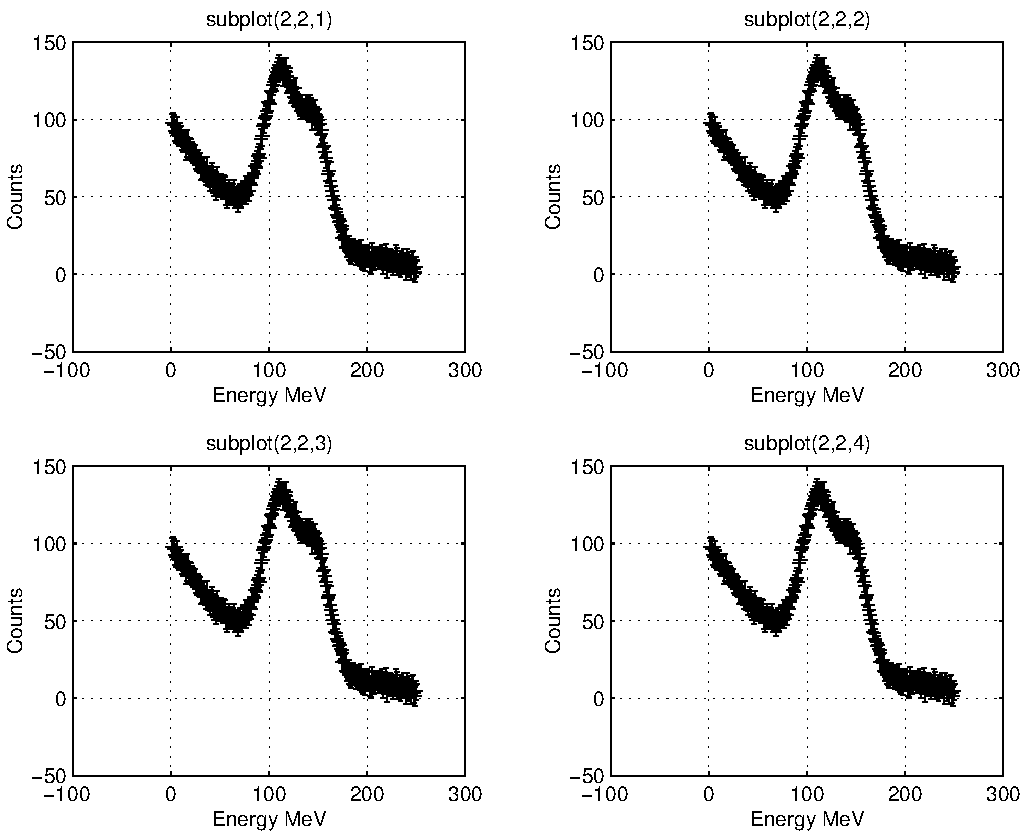
\includegraphics[width=20cm]{./figures/sample-fig5}
% \caption{For very large plots where important detail might be lost
% if too compressed. These full page graphics are usually best kept in
% appendices so as not to impede the flow of the paper.  Note that
% large tables can also be presented in this landscape environment if
% desired.} 
% \label{fig:landscapegraphic}
% \end{figure*}
% \end{turnpage}

% tables should appear as floats within the text
%
% Here is an example of the general form of a table:
% Fill in the caption in the braces of the \caption{} command. Put the label
% that you will use with \ref{} command in the braces of the \label{} command.
% Insert the column specifiers (l, r, c, d, etc.) in the empty braces of the
% \begin{tabular}{} command.
% The ruledtabular enviroment adds doubled rules to table and sets a
% reasonable default table settings.
% Use the table* environment to get a full-width table in two-column
% Add \usepackage{longtable} and the longtable (or longtable*}
% environment for nicely formatted long tables. Or use the the [H]
% placement option to break a long table (with less control than
% in longtable).
% \begin{table}%[H] add [H] placement to break table across pages
% \caption{\label{}}
% \begin{ruledtabular}
% \begin{tabular}{}
% Lines of table here ending with \\
% \end{tabular}
% \end{ruledtabular}
% \end{table}

% To convert program (e.g., C++ Fortran, Matlab, LaTeX\) listings to a
% form easily includable in a \LaTeX\ document
%
% type lgrind -s to see options
% lgrind -llatex -i sample-paper.tex > sampleinputtex
% creates a file sampleinput.tex which can then be included into this
% document simply by uncommenting the next line
%\lgrindfile{testinput.tex}

\section{Full Circuit Drawing of the Final Design}
\label{sec:fulldesign}

The final signal generator circuit schematic is presented in
Figure~\ref{fig:final_circuit}. The potentaial $v_t$ denotes the
$0-3.3$\unit{\volt} PWM signal modulating a $90$\unit{\hertz} sinusoidal wave at
a carrier frequency of $36.6$\unit{\kilo\hertz}. The potential $v_o$ denotes the
$0-10$\unit{\volt} analog $90$\unit{\hertz} sine-wave signal ready to be sent to
the Physik Instrumente controller as its reference input.

\begin{figure*}[b]
\begin{circuitikz}[scale=2, node distance=0.1mm and 0.1mm, rotate=-90, transform
    shape]
\draw (5,.5) node [op amp] (opamp) {\texttt{LM358}}
(opamp.down) -- ++(0,-0.25) node[ground] {}
(0,0) node [left] {$v_t$} to [R, l=$R_{d1}$, o-*] (2,0) node[below]{$v_m$} 
to [R, l=$R_{d2}$, *-*] (opamp.+)
to [C, l_=$C_{d2}$, *-] ($(opamp.+)+(0,-2)$) node [ground] {}
(opamp.out) |- (3.5,2) to [C, l_=$C_{d1}$, *-] (2,2) to [short] (2,0)
(opamp.-) -| (3.5,2)
% (opamp.out) to [short, *-*] (6.5,.5) node (vi) [above] {$v_i$};
(opamp.out) node (vi) [above right = of opamp.out]{$v_i$};
\draw[-latex] (opamp.up) -- ++(0,0.5) node [above] {$V_+$};

\draw (opamp.out) to[short, *-] ++(0.5,0) node[op amp, noinv input up, anchor=+]
(opamp2) {\texttt{LM358}}
(opamp2.-) -- ++(0, -2.0) coordinate (tmp) to [R, l=$R_{in}$, *-] ++(0,-2) node
[ground] (gnd) {} (tmp) to [R, l=$R_f$, -*] (tmp -| opamp2.out) -- (opamp2.out)
to [short, *-o] ++(1,0) node[above]{$v_o$};

\draw let 
    \p1 = (tmp), 
    \p2 = (opamp2.out)
    in
    (\x2, \y1) to [R, l=$R_{\text{load}}$] ++(0, -2) node[ground] {};

\draw (opamp2.down) -- ++(0,-0.25) node[ground] {};
\draw[-latex] (opamp2.up) -- ++(0,0.5) node [above] {$V_+$};

\end{circuitikz}
\caption{The final signal generator circuit design.}
\label{fig:final_circuit}
\end{figure*}



% \section{Just trial}
% 
% \begin{figure*}[t]
% \begin{circuitikz}[scale=0.9]
%     \draw (0,3) to[vsourcesin, name=vs] (0,6);
%     \node [below left, align=center, inner sep=12pt] at (vs.e)
%     {$0-3.3$\unit{\volt}\\$90$\unit{\hertz} PWM};
%     \node [right, align=center, inner sep=12pt] at (vs.e) {$v_t$};
%     \draw (0,6) to [R=$R$] (3,6) -- ++(0.0,0) node[label={above:$v_m$}] (vm) {}
%     to[short, *-] ++(0,0) to [C=$C$] (3,3) to node[ground]{} (3,3);
%     \node [ground] at (0,3) {};
% 
%     \draw (3,6) to[short, *-] ++(1.0,0) node[op amp, noinv input up, anchor=+](A1) {\texttt{OP292}};
% %     \draw (A1.+) to[short] (3,6);
%     \draw[-latex] (A1.up) -- ++(0,0.5) node [above] {$V_+$};
%     \draw (A1.down) -- ++(0,-0.25) node[ground] {};
%     \draw (A1.-) -- ++(0,-1.25) coordinate (tmp1);
%     \draw (A1.out) |- (tmp1);
% 
%     \draw (A1.out) to[short] ++(0.5,0) to [R=$R$] (8.5,5.51) -- ++(0.5,0)
%     node[label={above:$v_i$}] {} to[short, *-] ++(0.0,0)
%     to [C=$C$] (9,3) to [ground] (9, 3);
%     \node [ground] at (9.0, 3) {};
% 
%     \draw (9,5.51) to[short, *-] ++(1.0,0) node[op amp, noinv input up,
%     anchor=+](A2) {\texttt{OP292}}
%     (A2.-) -- ++(0, -2.0) coordinate (tmp2) to [R, l=$R_{in}$, *-] ++(0,-2) node
%     [ground] (gnd) {} (tmp2) to [R, l=$R_f$, -*] (tmp2 -| A2.out) -- (A2.out)
%     to [short, *-o] ++(1,0) node[above]{$v_o$};
% 
%     \draw let 
%     \p1 = (tmp2), 
%     \p2 = (A2.out)
%     in
%     (\x2, \y1) to [R, l=$R_{\text{load}}$] ++(0, -2) node[ground] {};
% 
%     \draw (A2.down) -- ++(0,-0.25) node[ground] {};
%     \draw[-latex] (A2.up) -- ++(0,0.5) node [above] {$V_+$};
% \end{circuitikz}
% \end{figure*}
% 
% 
% \begin{figure*}[b]
% \begin{circuitikz}[scale=1.5, node distance=0.1mm and 0.1mm, transform shape]
% \draw (5,.5) node [op amp] (opamp) {\texttt{OP292}}
% (opamp.down) -- ++(0,-0.25) node[ground] {}
% (0,0) node [left] {$v_t$} to [R, l=$R_{d1}$, o-*] (2,0) node[below]{$v_m$} 
% to [R, l=$R_{d2}$, *-*] (opamp.+)
% to [C, l_=$C_{d2}$, *-] ($(opamp.+)+(0,-2)$) node [ground] {}
% (opamp.out) |- (3.5,2) to [C, l_=$C_{d1}$, *-] (2,2) to [short] (2,0)
% (opamp.-) -| (3.5,2)
% % (opamp.out) to [short, *-*] (6.5,.5) node (vi) [above] {$v_i$};
% (opamp.out) node (vi) [above right = of opamp.out]{$v_i$};
% \draw[-latex] (opamp.up) -- ++(0,0.5) node [above] {$V_+$};
% 
% \draw (opamp.out) to[short, *-] ++(0.5,0) node[op amp, noinv input up, anchor=+]
% (opamp2) {\texttt{OP292}}
% (opamp2.-) -- ++(0, -2.0) coordinate (tmp) to [R, l=$R_{in}$, *-] ++(0,-2) node
% [ground] (gnd) {} (tmp) to [R, l=$R_f$, -*] (tmp -| opamp2.out) -- (opamp2.out)
% to [short, *-o] ++(1,0) node[above]{$v_o$};
% 
% \draw let 
%     \p1 = (tmp), 
%     \p2 = (opamp2.out)
%     in
%     (\x2, \y1) to [R, l=$R_{\text{load}}$] ++(0, -2) node[ground] {};
% 
% \draw (opamp2.down) -- ++(0,-0.25) node[ground] {};
% \draw[-latex] (opamp2.up) -- ++(0,0.5) node [above] {$V_+$};
% 
% \end{circuitikz}
% \end{figure*}

